\documentclass{article}

\usepackage[left=2cm,right=2cm,top=2cm,bottom=2cm]{geometry} 

\usepackage[utf8]{inputenc}   % otra alternativa para los caracteres acentuados y la "ñ"
\usepackage[           spanish % para poder usar el español
                      ,es-tabla % para los captions de las tablas
                       ]{babel}   
\decimalpoint %para usar el punto decimal en vez de coma para los números con decimales

%\usepackage{beton}
%\usepackage[T1]{fontenc}

\usepackage{parskip}
\usepackage{xcolor}

\usepackage{caption}

\usepackage{fancyvrb}

\usepackage{enumerate} % paquete para poder personalizar fácilmente la apariencia de las listas enumerativas

\usepackage{graphicx} % figuras
\usepackage{subfigure} % subfiguras

\usepackage{amsfonts}
\usepackage{amsmath}

\usepackage[formats]{listings}
\lstdefineformat{R}{~=\( \sim \)}
\lstset{basicstyle=\ttfamily,format=R}

\definecolor{gris}{RGB}{220,220,220}
	
\usepackage{float} % para controlar la situación de los entornos flotantes

\restylefloat{figure}
\restylefloat{table} 
\setlength{\parindent}{0mm}


\usepackage[bookmarks=true,
            bookmarksnumbered=false, % true means bookmarks in 
                                     % left window are numbered
            bookmarksopen=false,     % true means only level 1
                                     % are displayed.
            colorlinks=true,
            allcolors=blue,
            urlcolor=blue]{hyperref}
\definecolor{webblue}{rgb}{0, 0, 0.5}  % less intense blue


\title{\Huge SWAP: Servidor de disco NFS\vspace{10mm}}

\author{\huge David Cabezas Berrido \vspace{10mm} \\ 
  \huge dxabezas@correo.ugr.es \vspace{10mm}}

\begin{document}
\maketitle
\tableofcontents
\newpage

\section{Preparativos}

Creamos una nueva máquina virtual llamada \textbf{NFS-dxabezas}. Al igual que las otras máquinas, configuramos el doble adaptador de red
(NAT + Solo-Anfitrión), instalamos Ubuntu Server 18.04.1 y creamos un usuario \emph{dxabezas} con contraseña \emph{Swap1234}.
Comprobamos mediante PING que la máquina NFS tiene conexión con el resto de máquinas en la granja.

Su IP (en la red local) es \texttt{192.168.56.108}.

\section{Configurar servidor NFS}

Comenzamos creando la carpeta a compartir, y cambiamos el propietario y los permisos.

\begin{Verbatim}
sudo mkdir -p /datos/compartido
sudo chown nobody:nogroup /datos/compartido/
sudo chmod -R 777 /datos/compartido/
\end{Verbatim}

Comprobamos el propietario y los permisos que acabamos de asignar.

\begin{figure}[H]
	\centering
	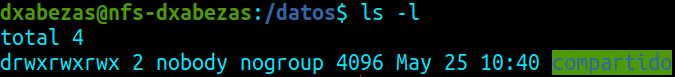
\includegraphics[width=110mm]{imgs/compartido-ls-l}
\end{figure}

Le damos permisos a M1 y M2 añadiendo la siguiente línea a \texttt{/etc/exports}.
\begin{Verbatim}
/datos/compartido/ 192.168.56.102(rw) 192.168.56.101(rw)
\end{Verbatim}

Finalmente, reiniciamos el servicio y comprobamos el estado.
\begin{figure}[H]
	\centering
	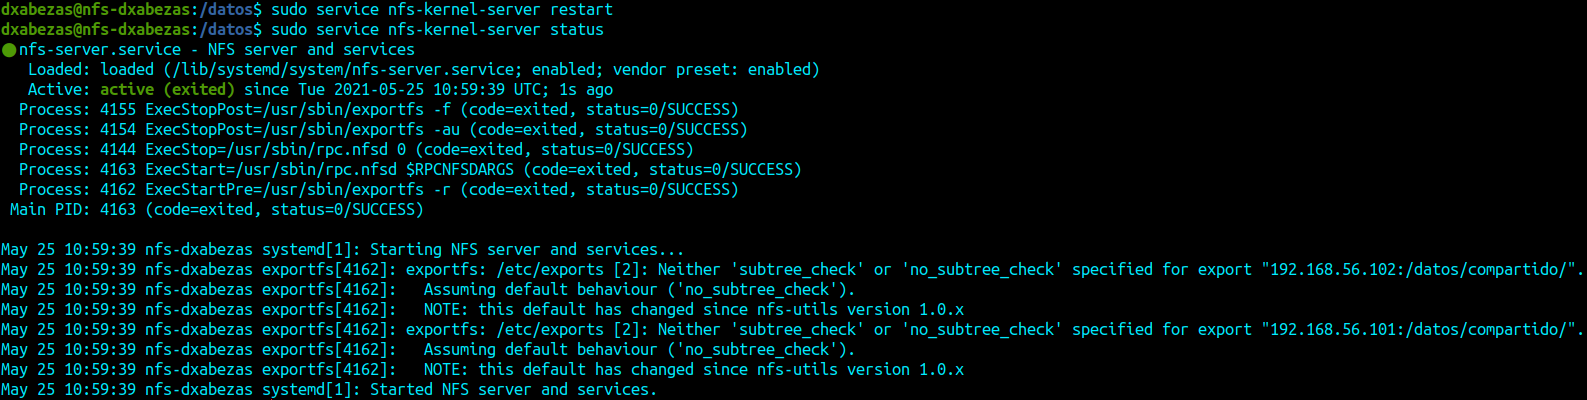
\includegraphics[width=180mm]{imgs/status}
	\caption{Todo parece estar correcto, teniendo en cuenta que estamos asumiendo la opción \texttt{no\_subtree\_check}. El subtree check consiste
	en comprobar que cada petición NFS solicita sólo archivos que están siendo exportados, para ello necesita información sobre el directorio
	padre.}
\end{figure}

\section{Configurar los clientes M1 y M2}

La siguiente configuración se realiza tanto en M1 como en M2.

Primero instalamos los paquetes necesarios.
\begin{Verbatim}
sudo apt install nfs-common rpcbind
\end{Verbatim}

A continuación, creamos el punto de montaje, el directorio \texttt{datos}. También le damos todos los permisos sobre él a todos los usuarios.
\begin{Verbatim}
cd /home/dxabezas
mkdir datos
chmod -R 777 datos
\end{Verbatim}

Si ahora modificamos la carpeta compartida en alguna máquina (M1, M2 o servidoro NFS), los cambios también se hacen efectivos en las otras dos.
\begin{figure}[H]
	\centering
	\subfigure{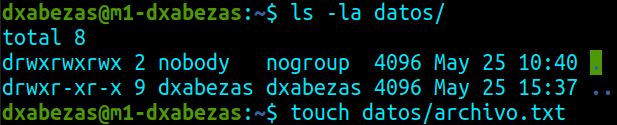
\includegraphics[width=90mm]{imgs/m1-touch}}
	\subfigure{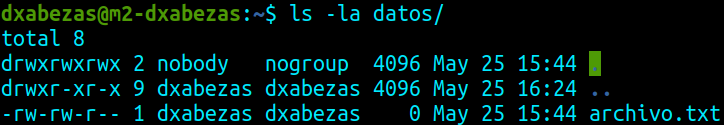
\includegraphics[width=100mm]{imgs/m2-ls}}
	\subfigure{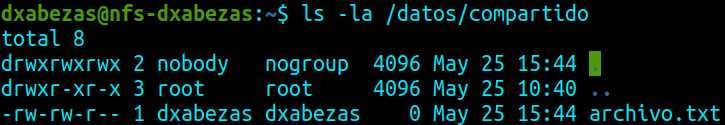
\includegraphics[width=100mm]{imgs/nfs-ls}}
	\caption{El archivo creado por M1 aparece en M2 y en el servidor NFS.}
	\label{fig:test}
\end{figure}

\subsection{Hacer la configuración permanente}

Para hacer la configuración permanente, sólo tenemos que añadir (tanto en M1 como en M2) la siguiente línea al fichero \texttt{/etc/fstab}.
\begin{Verbatim}[tabsize=4]
192.168.56.108:/datos/compartido /home/dxabezas/datos/ nfs
	auto,noatime,nolock,bg,nfsvers=3,intr,tcp,actimeo=1800 0 0
\end{Verbatim}
Al reiniciar la máquina, comprobamos que el directorio está montado y podemos acceder a los archivos.

\section{Seguridad en el servidor NFS}

Nuestro objetivo es configurar IPTABLES para que el servidor NFS siga funcionando mientras denegamos implícitamente el tráfico entrante.
Partimos por tanto de la siguiente configuración:
\begin{Verbatim}
iptables -P INPUT DROP
iptables -P OUTPUT ACCEPT
iptables -P FORWARD DROP
iptables -A INPUT -m state --state ESTABLISHED,RELATED -j ACCEPT
\end{Verbatim}

Para los servicios \textbf{nfs} y \textbf{portmapper}, sólo tenemos que abrir los puertos 2049 y 111 respectivamente, tanto TCP como UDP.
Sin embargo, los servicios \textbf{mountd} y \textbf{nlockmgr} utilizan puertos dinámicos. Podemos consultar qué puerto está utilizando cada servicio
con la siguiente orden.

\begin{figure}[H]
	\centering
	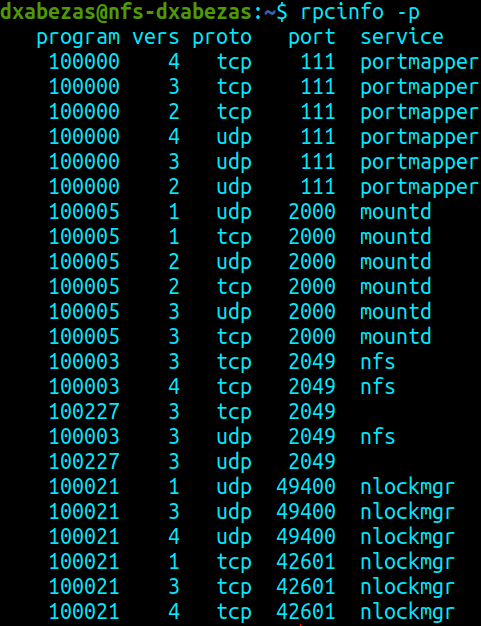
\includegraphics[width=80mm]{imgs/rpcinfo1}
\end{figure}

Como no podemos abrir puertos dinámicamente con IPTABLES, fijaremos puertos para estos servicios. Para \textbf{mountd}, modificamos el archivo
\texttt{/etc/default/nfs-kernel-server} y añadimos la siguiente línea.
\begin{Verbatim}
RPCMOUNTDOPTS="--manage-gids -p 2000"
\end{Verbatim}
Para \textbf{nlockmgr}, creamos el archivo \texttt{/etc/sysctl.d/swap-nfs-ports.conf} con las siguientes opciones
\begin{Verbatim}
fs.nfs.nlm_tcpport = 2001
fs.nfs.nlm_udpport = 2002
\end{Verbatim}

Lanzamos el archivo de configuración y reniciamos el servidor NFS con las siguientes órdenes.
\begin{Verbatim}
sudo sysctl --system
/etc/init.d/nfs-kernel-server restart
\end{Verbatim}
La primera de ellas devuelve una salida muy extensa de configuraciones que se aplican. Entre ellas, está la siguiente secuencia.
\begin{Verbatim}
* Applying /etc/sysctl.d/swap-nfs-ports.conf ...
fs.nfs.nlm_tcpport = 2001
fs.nfs.nlm_udpport = 2002
\end{Verbatim}
La segunda orden produce la siguiente salida.
\begin{Verbatim}
[ ok ] Restarting nfs-kernel-server (via systemctl): nfs-kernel-server.service.
\end{Verbatim}

Como parece que todo va correctamente, volvemos a comprobar los puertos que utiliza cada servicio.

\begin{figure}[H]
	\centering
	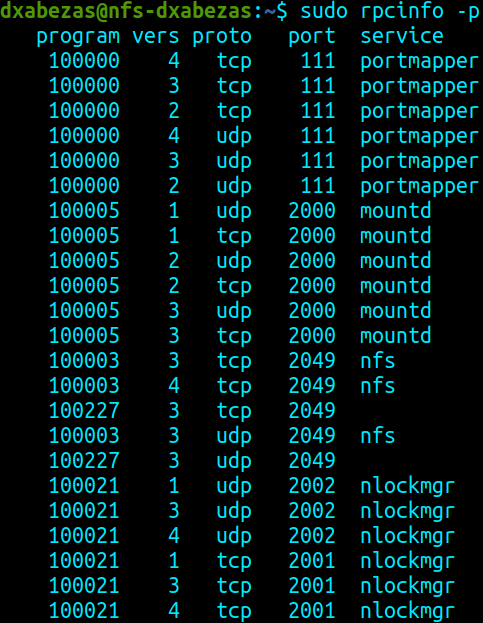
\includegraphics[width=80mm]{imgs/rpcinfo2}
\end{figure}

Como podemos observar, son justo los puertos que hemos seleccionado. Ahora podemos abrirlos con IPTABLES (sólo para M1 y M2) como solemos hacer.
Nuestro script de IPTABLES queda de esta forma.

\begin{Verbatim}
#!/bin/sh

# 1: Eliminar todas las reglas, configuración limpia
iptables -F
iptables -X
iptables -Z

# 2: Denegación implícita del tráfico entrante
iptables -P INPUT DROP
iptables -P OUTPUT ACCEPT
iptables -P FORWARD DROP

# 3: Permitir conexiones
iptables -A INPUT -m state --state ESTABLISHED,RELATED -j ACCEPT

# 4: Permitir acceso desde localhost (interface lo):
iptables -A INPUT -i lo -j ACCEPT
iptables -A OUTPUT -o lo -j ACCEPT

# 5: Abrir puerto 2049 (nfs), TCP y UDP, sólo M1 y M2
iptables -A INPUT -p tcp -s 192.168.56.102 --dport 2049 -j ACCEPT
iptables -A INPUT -p udp -s 192.168.56.102 --dport 2049 -j ACCEPT
iptables -A INPUT -p tcp -s 192.168.56.101 --dport 2049 -j ACCEPT
iptables -A INPUT -p udp -s 192.168.56.101 --dport 2049 -j ACCEPT

# 6: Abrir puerto 111 (portmapper), TCP y UDP, sólo M1 y M2
iptables -A INPUT -p tcp -s 192.168.56.102 --dport 111 -j ACCEPT
iptables -A INPUT -p udp -s 192.168.56.102 --dport 111 -j ACCEPT
iptables -A INPUT -p tcp -s 192.168.56.101 --dport 111 -j ACCEPT
iptables -A INPUT -p udp -s 192.168.56.101 --dport 111 -j ACCEPT

# 7: Abrir puerto 2000 (mountd), TCP y UDP, sólo M1 y M2
iptables -A INPUT -p tcp -s 192.168.56.102 --dport 2000 -j ACCEPT
iptables -A INPUT -p udp -s 192.168.56.102 --dport 2000 -j ACCEPT
iptables -A INPUT -p tcp -s 192.168.56.101 --dport 2000 -j ACCEPT
iptables -A INPUT -p udp -s 192.168.56.101 --dport 2000 -j ACCEPT

# 8: Abrir puertos para nlockmgr: 2001 (TCP) y 2002 (UDP), sólo M1 y M2
iptables -A INPUT -p tcp -s 192.168.56.102 --dport 2001 -j ACCEPT
iptables -A INPUT -p udp -s 192.168.56.102 --dport 2002 -j ACCEPT
iptables -A INPUT -p tcp -s 192.168.56.101 --dport 2001 -j ACCEPT
iptables -A INPUT -p udp -s 192.168.56.101 --dport 2002 -j ACCEPT
\end{Verbatim}

Activamos esta configuración. Para comprobar que sigue funcionando, realizamos satisfactoriamente una modificación similar a la de la Figura \ref{fig:test},
modificando también desde M1.

\end{document}
